\section{Durchführung}
\label{sec:Durchführung}

Aus Zeitgründen und aufgrund der durch das Corona-Virus bedingten Umstrukturierung der Praktikumsrahmenbedingungen 
wird nicht die Ionisierungsenergie der Hg-Atome gemessen; es werden ausschließlich die Energieverteilung der Elektronen 
und die Anregungsenergie betrachtet. Außerdem wird die Zahl der Messreihen reduziert. 

\begin{figure}
    \centering
    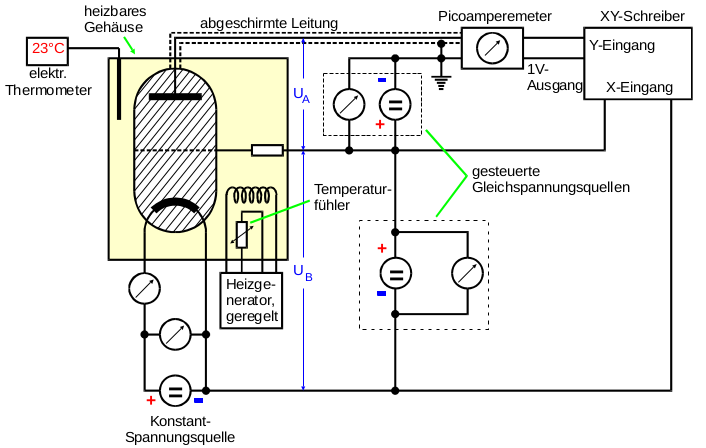
\includegraphics[width=\textwidth]{plots/Aufbau.png}
    \caption{Der Versuchsaufbau\cite{Versuchsanleitung}.}
    \label{fig:Aufbau}
\end{figure}
In Abbildung \ref{fig:Aufbau} ist der Versuchsaufbau zu sehen. 
Die erwähnte Franck--Hertz-Röhre ist in einem heizbaren Gehäuse untergebracht. Die Temperatur kann an dem elektrischen 
Thermometer abgelesen und über einen Heizgenerator geregelt werden. 
Das Picoamperemeter misst den Auffängerstrom $I_\text{A}$.
Ein XY-Schreiber kann die Franck--Hertz-Kurve aufzeichnen. Dafür werden an den X- und Y-Eingang jeweils die Spannungen 
gegeben, die der Abszisse (X) und Ordinate (Y) zugeordnet werden sollen. 
Das Picoamperemeter ist in der Lage, eine dem Auffängerstrom proportionale Spannung bereitzustellen, sodass auch der 
Strom graphisch dargestellt werden kann. 
Das Millimeterpapier lässt sich elektrostatisch auf dem Schreiber fixieren, sodass dieses nicht bei der Aufzeichnung verrutscht. 

Die Eichung und Regulierung der Achsen an dem XY-Schreiber sind intuitiv und größtenteils selbsterklärend. 
Hier muss beachtet werden, dass beim maximalen Strom ($U_\text{A}=\SI{0}{\volt}$) der Schreiber nur knapp bis zum 
Anschlag wandert, und dass die X-Achse mit zugehörigen Spannungswerten versehen werden muss, um später quantitative Ergebnisse 
ablesen zu können. 
\\

Zuerst wird die sogenannte integrale Energieverteilung der Elektronen gemessen. Die Beschleunigungsspannung wird hierfür auf 
einen konstanten Wert von $\SI{11}{\volt}$ eingestellt und der Auffängerstrom unter Erhöhung der Bremsspannung mit 
dem Schreiber aufgezeichnet. 
Der bei $U_\text{A}=\SI{0}{\volt}$ fließende Strom wird mithilfe der Glühkathodenspannung auf einen Wert zwischen $50$ und $\SI{500}{\nano\ampere}$
eingestellt. 

Diese Messung wird zuerst für Raumtemperatur durchgeführt, im Anschluss für eine höhere Temperatur von etwa $\SI{150}{\degreeCelsius}$. 
Dieser letzte Schritt entfällt jedoch aus genannten Gründen. 

Beim nächsten Messschritt wird ebenfalls nur eine Messreihe aufgenommen. 
Diesmal wird der Auffängerstrom in Abhängigkeit der Beschleunigungsspannung gemessen, um eine Franck--Hertz-Kurve zu erhalten. 
Die Bremsspannung wird auf etwa $\SI{1}{\volt}$ konstant gehalten. 
Die Temperatur soll hier idealerweise im Intervall $160$ bis $\SI{200}{\degreeCelsius}$ liegen. 
Die Beschleunigungsspannung kann auf maximal $\SI{60}{\volt}$ eingestellt werden. 
Durch Ausprobieren wird festgestellt, bis zu welchem Spannungswert eine Aufzeichnung des Auffängerstroms sinnvoll ist, 
da irgendwann die Strommaxima nicht mehr gut gemessen werden können, und wie entsprechend die X-Achse des XY-Schreibers 
geeicht werden muss. 

Als letzter Schritt würde die Messung der Ionisierungsenergie folgen; hierzu würde die Temperatur auf etwa $100$ bis $\SI{110}{\degreeCelsius}$ 
geregelt werden und die Bremsspannung auf $\SI{30}{\volt}$.